
Many physics analyses seek final states with particles that are weakly
interacting and just pass through the detector undetected. Because the
initial momenta of the incoming partons is approximately zero in the
transverse plane, the presence of these undetected particles can be
inferred by measuring the missing momentum in this
direction. Mathematically, this is seen by requiring momentum conservation

\begin{equation}
\begin{aligned}
\vect{p}^{\textrm{incoming}}_{\textrm{T}} = 0 &=
\vect{p}^{\textrm{outgoing}}_{\textrm{T}} \\
&= \vect{p}^{\textrm{visible}}_{\textrm{T}} +
\vect{p}^{\textrm{missing}}_{\textrm{T}}, 
\end{aligned}
\end{equation}

\noindent
which implies that $\vect{p}^{\textrm{missing}}_{\textrm{T}}$ is
obtained by measuring
$-\vect{p}^{\textrm{visible}}_{\textrm{T}}$. Since the longitudinal momenta of the
incoming partons is not known, this quantity can not be inferred
through momentum conservation, making it impossible to reconstruct the
4-momentum of the undetected particles. In this thesis, the missing transverse
momentum of the visible particles
$\vect{p}^{\textrm{visible}}_{\textrm{T}}$ is reconstructed using
either calorimeter deposits or tracks. The former is denoted \calomet
while the latter is denoted \trkmet. Generically, missing transverse
energy will be referred to as \etmiss.

\subsection{Calorimeter \etmiss Reconstruction}

Calorimeter-based missing transverse energy uses information from the
calorimeter as well as the tracking systems for muons, and can
therefore be decomposed into two terms~\cite{bib:ATLAS-CONF-2013-082}. The calorimeter term is
further decomposed into the high-\pt~ physics objects which are
reconstructed from calorimeter information, as well as a soft term for
the low energy deposits not associated to a high-\pt object:

\begin{equation}
\vect{\ensuremath{E}}_{\mathrm{T}}^{\mathrm{miss, CALO}} =
\vect{\ensuremath{E}}_{\mathrm{T}}^{\mathrm{miss},e} +
\vect{\ensuremath{E}}_{\mathrm{T}}^{\mathrm{miss},\gamma} +
\vect{\ensuremath{E}}_{\mathrm{T}}^{\mathrm{miss},\tau} +
\vect{\ensuremath{E}}_{\mathrm{T}}^{\mathrm{miss,jets}} +
\vect{\ensuremath{E}}_{\mathrm{T}}^{\mathrm{miss,soft}} + 
\vect{\ensuremath{E}}_{\mathrm{T}}^{\mathrm{miss},\mu}
\label{chap:reco:equation:etmiss}
\end{equation}

\noindent
To avoid double-counting energy in the calorimeter, selection of the
objects going into equation~\ref{chap:reco:equation:etmiss} is done
sequentially. First, the
$\vect{\ensuremath{E}}_{\mathrm{T}}^{\mathrm{miss},e}$ term is defined
using reconstructed electrons (section~\ref{chap:reco:sec:electron})
with $\pt > 10 \gev$ (what kind of electrons?). Then photons with $\pt
> 10 \gev$ and without any overlap with reconstructed electrons are
selected. High-\pt~jets ($\pt > 20 \gev$) are reconstructed with
topological clusters using the \antikt algorithm with distance measure
$R=0.4$ (section~\ref{chap:reco:sec:jet}). These clusters are required
to be isolated from those associated to electrons or photons. To reject jets from
pile-up, jets with $|\eta| < 2.4$ and $20~\gev < \pt < 50~\gev$ are
required to have $|\textrm{JVF}| > 0$
(section~\ref{chap:reco:sec:jet:subsec:quality}) (I don't think this
is the case for METRefFinal). The final calorimeter term represents
energy in the event that is not associated with high-\pt~objects. This
soft term is built from LCW-calibrated topological clusters which do
not have an explicit $E_T$ requirement but are robust against
electronic and pileup noise
(section~\ref{chap:reco:sec:cluster}. Given that it is not possible to
reliably match a cluster to a primary vertex, the soft term is highly sensitive
to in-time pileup, as shown in
figure~\ref{chap:reconstruction:fig:softterm_pileup}. In an inclusive
$Z\rightarrow{\mu\mu}$ sample, the average soft term at $\nvtx = 1$ is
around $10 \gev$ and increases to $40 \gev$ at $\nvtx = 25$. This
term significantly degrades both the magnitude and direction
resolutions for \etmiss. Various corrections which help to mitigate
the dependence on pileup have been used in
ATLAS~\cite{bib:ATLAS-CONF-2014-019}, but for the analysis presented
in this thesis, the baseline calorimeter \etmiss definition without
corrections is used. 

\begin{figure}[h]
    \centering
    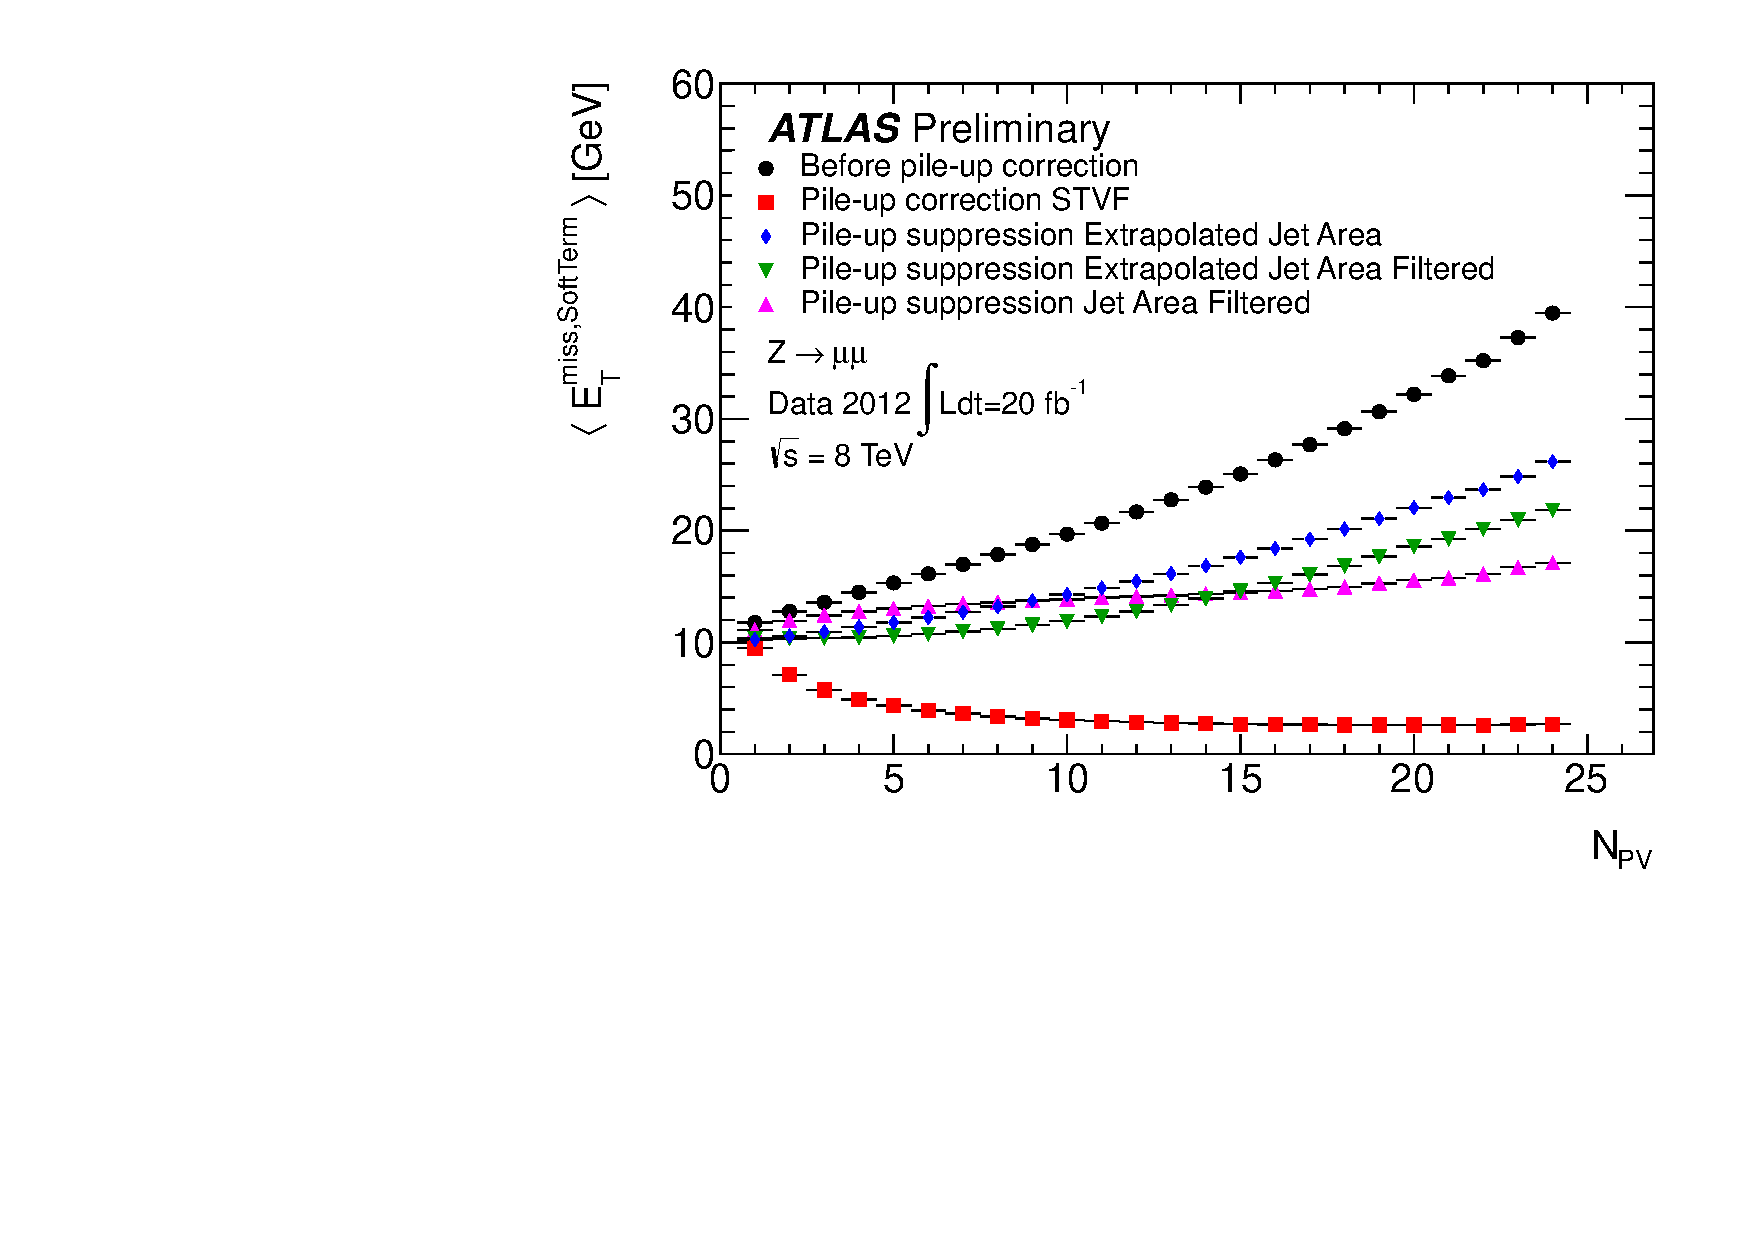
\includegraphics[width=0.6\textwidth]{fig/reconstruction/cell_out_PU_Zmumu.pdf}
    \caption[]{The average calorimeter \etmiss soft term $\left \langle
      E_{\mathrm{T}}^{\mathrm{miss,soft}} \right \rangle$ (shown in black) as a
      function of the number of primary vertices for an inclusive $Z\rightarrow{\mu\mu}$
      sample in $\sqrts=8 \tev$ data~\cite{bib:ATLAS-CONF-2014-019}.}
\label{chap:reconstruction:fig:softterm_pileup}
\end{figure}

For the
muon term, combined muons (section~\ref{chap:reco:sec:muon}) with $\pt
> 6~\gev$ are used
where there is both ID and MS coverage ($0.1 < |\eta| < 2.5$). Because
muons usually leave energy clusters in the calorimeter, and the
combined muon fit accounts for this loss, the combined muon energy is
double-counted. This is corrected by subtracting the parameterized energy loss in the
calorimeter from the fitted muon momentum. Outside of the ID,
standalone muons are used, while in regions with limited MS coverage
($|\eta| < 0.1$), ID track muons are used.

\subsection{Track \etmiss Reconstruction}

As mentioned in the previous section, \calomet is sensitive to in-time
pileup, degrading its resolution for large \nvtx events. Track \etmiss
seeks to suppress pileup dependence by replacing the clusters defining
the soft term with tracks matched to the primary vertex of the
event (section~\ref{chap:reco:sec:tracks}. These tracks are required
to have $\pt > 500 \mev$ and $|\eta| < 2.5$, with additional quality
requirements: $|d_0 < 1.5$~mm, $|z_0\sin(\theta) < 1.5$~mm,
$N_{\textrm{hits}}^{\textrm{pixel}} \geq 1$, and
$N_{\textrm{hits}}^{\textrm{SCT}} \geq 6$. If a track fails these
quality criteria, but pass requirements associated with electrons and
muons, then the associated leptons \pt~replaces the track. The lepton
requirements are similar to those in the \calomet definition, with
some important exceptions which will be discussed in
chapter~\ref{chap:analysis}. Moreover, tracks that fall within a cone
of $R=0.4$ of a jet are not included in \etmiss; instead the jet
itself is used. The rationale is that
if tracks are used to define \etmiss instead of reconstructed jets,
neutral tracks associated with the jets are missed, thereby degrading
the \etmiss resolution. The specific definition of a jet is
analysis-dependent, and will therefore be described in detail in
chapter~\ref{chap:analysis}. 
